\documentclass[12pt]{article}
\AddToHook{cmd/section/before}{\clearpage}

\usepackage{microtype}
\usepackage{polyglossia}
\setmainlanguage{italian}

\usepackage{fontspec}
\setmainfont{Old Standard}

\usepackage{unicode-math}
\unimathsetup{math-style=ISO}
\setmathfont{Latin Modern Math}

\usepackage[locale=IT]{siunitx}

\usepackage[pdfusetitle]{hyperref}
\hypersetup{%
    linktoc       = all,
    pdfdirection  = L2R,
    pdfkeywords   = {Reti logiche, VHDL},
    pdflang       = it,
    pdfpagelayout = OneColumn,
    pdfsubject    = {Reti logiche}
}

\usepackage{rotating}
\usepackage{tikz}
\usetikzlibrary{arrows.meta, automata, calc, positioning}

\author{Matteo Delton \and Gianluca Di Paola}
\title{Progetto di reti logiche}
\date{a.a.~2023/2024}

\begin{document}

\begin{titlepage}
    \centering
    \includegraphics[width=0.75\textwidth]{polimi_logo_vertical.pdf}

    \vspace{1cm}

    {\Huge\textbf{Prova finale}\par}
    {\LARGE Progetto di reti logiche\par}
    \vspace{0.5cm}
    Professore: \\
    {\large William Fornaciari\par}

    \vspace{1.5cm}

    Relazione di: \\
    {\large Matteo Delton (\texttt{10786485}) \\ Gianluca Di Paola (\texttt{10797584})\par}

    \vfill
    a.a.~2023/2024
\end{titlepage}

\tableofcontents

\section{Introduzione}

Il progetto di reti logiche per l'anno accademico 2023/2024 consiste nella realizzazione di un modulo hardware nel linguaggio VHDL che si interfacci con una RAM\@, come mostrato in figura~\ref{fig:high_level}.

\begin{figure}[hb]
    \centering
    \begin{tikzpicture}[
            >=Stealth,
            shorten >=1pt,
            auto,
            semithick
        ]
        \node [draw, rectangle, minimum width=7cm, minimum height=4cm] (module) at (0, 0) {Modulo};
        \node [draw, rectangle, minimum width=7cm, minimum height=1cm, above=3cm of module] (ram) {RAM};

        % Clock and reset signals
        \draw[->] ($(module.south) + (-1, -1.5)$) node[below] {\texttt{i\_clk}} to ($(module.south west)!(\tikztostart)!(module.south east)$);
        \draw[->] ($(module.south) + (1, -1.5)$) node[below] {\texttt{i\_rst}} to ($(module.south west)!(\tikztostart)!(module.south east)$);

        % Input signals
        \draw[->] ($(module.west) + (-1.5, 1)$) node[left] {\texttt{i\_start}} to ($(module.north west)!(\tikztostart)!(module.south west)$);
        \draw[->] ($(module.west) + (-1.5, 0)$) node[left] {\texttt{i\_add}} to coordinate (i_add_m) (module.west);
        \draw[->] ($(module.west) + (-1.5, -1)$) node[left] {\texttt{i\_k}} to coordinate (i_k_m) ($(module.south west)!(\tikztostart)!(module.north west)$);

        \draw ($(i_add_m) + (-0.1, -0.1)$) to node[above, font=\scriptsize] {\(16\)} ++(0.2, 0.2);
        \draw ($(i_k_m) + (-0.1, -0.1)$) to node[above, font=\scriptsize] {\(10\)} ++(0.2, 0.2);

        % RAM signals
        \draw[->] ($(module.north) + (-2.5, 0)$) to node[rotate=90, above] {\texttt{o\_mem\_addr}} coordinate (o_mem_addr_m) ($(ram.south west)!(\tikztostart)!(ram.south east)$);
        \draw[->] ($(ram.south) + (-1.25, 0)$)   to node[rotate=90, above] {\texttt{i\_mem\_data}} coordinate (i_mem_data_m) ($(module.north west)!(\tikztostart)!(module.north east)$);
        \draw[->] (module.north)                 to node[rotate=90, above] {\texttt{o\_mem\_data}} coordinate (o_mem_data_m) (ram.south);
        \draw[->] ($(module.north) + (1.25, 0)$) to node[rotate=90, above] {\texttt{o\_mem\_we}} ($(ram.south west)!(\tikztostart)!(ram.south east)$);
        \draw[->] ($(module.north) + (2.5, 0)$)  to node[rotate=90, above] {\texttt{o\_mem\_en}} ($(ram.south west)!(\tikztostart)!(ram.south east)$);

        \draw ($(o_mem_addr_m) + (-0.1, -0.1)$) to node[right, font=\scriptsize] {\(16\)} ++(0.2, 0.2);
        \draw ($(i_mem_data_m) + (-0.1, -0.1)$) to node[right, font=\scriptsize] {\(8\)} ++(0.2, 0.2);
        \draw ($(o_mem_data_m) + (-0.1, -0.1)$) to node[right, font=\scriptsize] {\(8\)} ++(0.2, 0.2);

        % Output signals
        \draw[->] (module.east) to ++(1.5, 0) node[right] (o_done) {\texttt{o\_done}};
    \end{tikzpicture}
    \caption{Rappresentazione di alto livello del modulo}\label{fig:high_level}
\end{figure}

Il modulo ha il compito di completare una sequenza a partire da un indirizzo di memoria \(\textup{ADD}\) dato.

La sequenza è composta da \(K\) coppie di elementi di 8~bit ciascuno: il primo elemento identifica la ``parola'' \(W\) in ingresso, mentre il secondo sarà codificato nel suo ``valore di credibilità'' \(C\).

Le parole hanno un valore compreso tra \(0\) e \(255\). Il valore \(0\) codifica l'informazione di ``valore non specificato''; il modulo sostituisce tutte le parole di valore \(0\) con l'ultima parola letta di valore diverso da \(0\) (o con \(0\) se non ce ne sono mai state).

I valori di credibilità \(C\) hanno un valore compreso tra \(0\) e \(31\) e sono calcolati dal modulo come segue:
\begin{itemize}
    \item se la parola ha un valore specificato (ovvero, è diversa da \(0\)), il suo valore di credibilità sarà il massimo \(31\);
    \item se la parola \emph{non} ha un valore specificato (ovvero, se è \(0\)), il suo valore di credibilità sarà pari al valore di credibilità della parola precedente decrementato di \(1\), salvo se questo vale \(0\), nel qual caso non viene ulteriormente decrementato. Qualora non ci sia una parola precedente, il valore di credibilità è posto a \(0\).
\end{itemize}

Volendo ricavare una regola generale di funzionamento, noto l'indirizzo \(\textup{ADD}\) della prima parola (fornito a inizio computazione), la parola \(i\)-esima \(W_{i}\) della sequenza si troverà all'indirizzo di memoria \(\textup{ADD} + 2(i - 1)\) e il suo valore di credibilità \(C_i\) la seguirà all'indirizzo \(\textup{ADD} + 2(i - 1) + 1\).

Il modulo deve essere in grado di riconoscere un segnale di reset \texttt{i\_rst} asincrono, che può essere ricevuto in un qualsiasi momento.
Ogni nuova computazione inizia con l'arrivo di un segnale alto \texttt{i\_start}, che può essere ricevuto solo al termine di una elaborazione precedente e può (ma non deve necessariamente) essere preceduto da \texttt{i\_rst} (lo è certamente alla prima computazione). Tale segnale \texttt{i\_start} rimane alto mentre il modulo è attivo.
Al termine dell'elaborazione, il modulo alza il segnale di \texttt{o\_done}; quindi, non appena riconosce l'abbassamento di \texttt{i\_start}, porta basso \texttt{o\_done}.

\section{Architettura}

Per la sintesi del modulo, è stato usato il software Xilinx Vivado con una FPGA target Artix-7 xc7a200tfbg484-1. Abbiamo adottato il paradigma di progettazione \textit{behavioral}.

Il componente è stato implementato attraverso una macchina a stati finiti (FSM), composta da tre processi principali (descritti in seguito) per rendere più atomica la struttura del modulo e facilitare la gestione complessiva. La FSM è formata da dieci stati, come mostrato in figura~\ref{fig:fsm}.

\subsection{Stati della FSM}

\begin{figure}[ht]
    \centering
    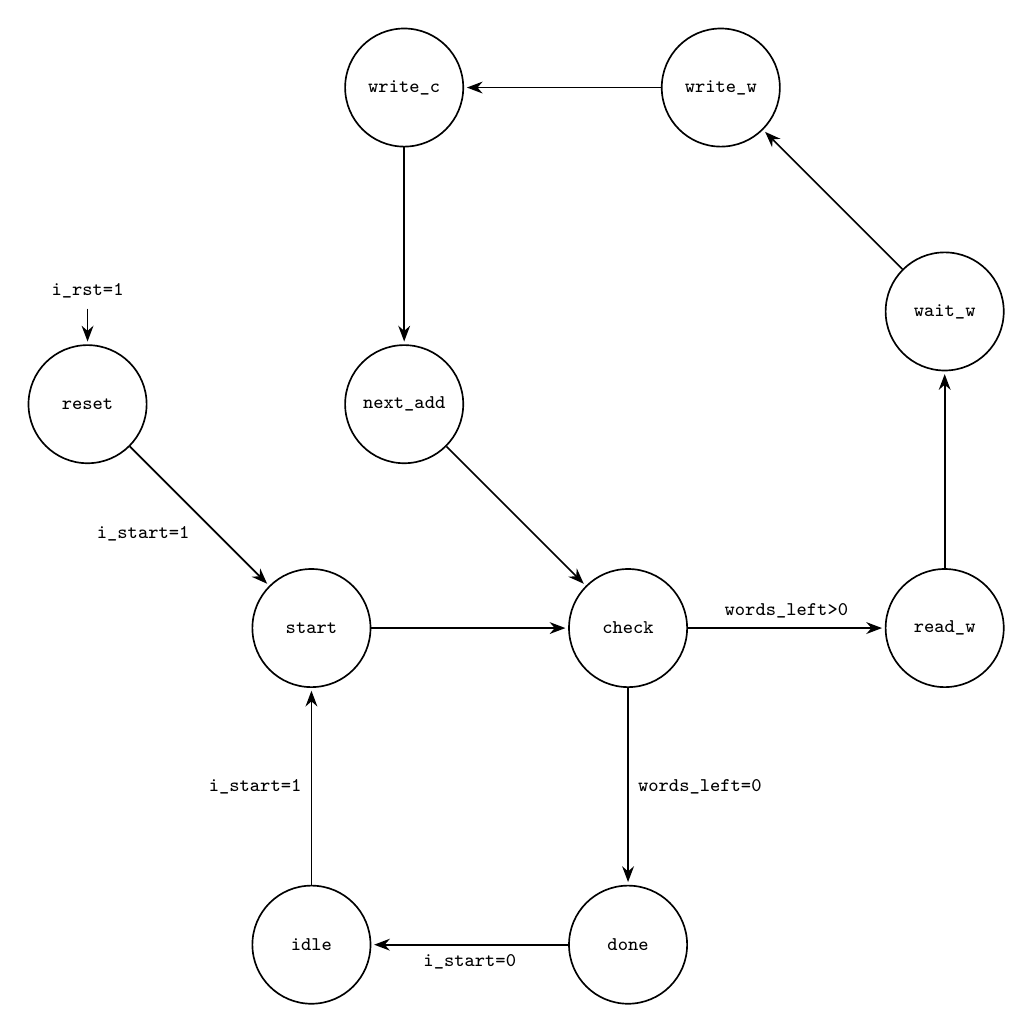
\begin{tikzpicture}[
            ->,
            >=Stealth,
            shorten >=1pt,
            auto,
            node distance=2.5cm,
            semithick,
            initial text=\texttt{i\_rst=1}
        ]
        \tikzstyle{every state}=[fill=white,draw=black,text=black, minimum size=1.5cm, font=\scriptsize]
        \tikzstyle{every edge}=[font=\scriptsize, draw=black]

        \node[state, initial above] (S1) {\texttt{reset}};
        \node[state] (S2) [below right=of S1] {\texttt{start}};
        \node[state] (S3) [right=of S2] {\texttt{check}};
        \node[state] (S4) [right=of S3] {\texttt{read\_w}};
        \node[state] (S5) [above=of S4] {\texttt{wait\_w}};
        \node[state] (S6) [above left=of S5] {\texttt{write\_w}};
        \node[state] (S7) [left=of S6] {\texttt{write\_c}};
        \node[state] (S8) [below=of S7] {\texttt{next\_add}};
        \node[state] (S9) [below=of S3] {\texttt{done}};
        \node[state] (S10) [left=of S9] {\texttt{idle}};

        \path (S1) edge node [swap] {\texttt{i\_start=1}} (S2)
        (S2) edge (S3)
        (S3) edge node {\texttt{words\_left>0}} (S4)
        (S4) edge (S5)
        (S5) edge (S6)
        (S6) edge (S7)
        (S7) edge (S8)
        (S8) edge (S3)
        (S3) edge node {\texttt{words\_left=0}} (S9)
        (S9) edge node {\texttt{i\_start=0}} (S10)
        (S10) edge node {\texttt{i\_start=1}} (S2);
    \end{tikzpicture}
    \caption{Diagramma degli stati della FSM}\label{fig:fsm}
\end{figure}

Di seguito una descrizione degli stati:
\begin{itemize}
    \item \texttt{reset}: stato in cui si trova il modulo, a seguito del segnale di reset asincrono, in cui tutti i segnali sono posti a zero. Tale stato è raggiungibile da tutti gli altri stati in qualsiasi momento della computazione;
    \item \texttt{start}: stato in cui, letti la lunghezza della sequenza e il suo indirizzo iniziale, vengono inizializzati i contatori. La FSM entra in questo stato a seguito di \texttt{i\_start} alto;
    \item \texttt{check}: stato in cui il modulo verifica se ci sono ancora parole da processare. Abbiamo deciso di inserirlo immediatamente dopo \texttt{start} per gestire il caso in cui la sequenza sia vuota (lunghezza \texttt{i\_k} pari a zero)\footnote{Anche se in una comunicazione è stato chiarito che la lunghezza della sequenza non può essere nulla, abbiamo deciso di gestire comunque questo caso per completezza.};
    \item \texttt{read\_w}: stato in cui il modulo richiede la parola in lettura alla RAM;
    \item \texttt{wait\_w}: stato in cui il modulo attende che la parola richiesta sia disponibile;
    \item \texttt{write\_w}: stato in cui il modulo imposta il valore di credibilità e sovrascrive, se necessario, il valore di una parola non specificata. Viene anche fornito l'indirizzo della parola in questione;
    \item \texttt{write\_c}: stato in cui il modulo scrive il valore di credibilità. Viene anche fornito l'indirizzo del valore di credibilità in questione;
    \item \texttt{next\_add}: stato in cui il modulo aggiorna l'indirizzo di memoria salvato e decrementa il contatore delle parole rimanenti;
    \item \texttt{done}: stato in cui il modulo segnala la fine della computazione, alzando \texttt{o\_done}. La FSM entra in questo stato solo quando non ci sono altre parole da elaborare;
    \item \texttt{idle}: stato in cui il modulo abbassa \texttt{o\_done} e resta in attesa di un nuovo segnale \texttt{i\_start} alto per iniziare una nuova computazione (a quel punto la FSM va nello stato \texttt{start}). Si entra in questo stato solo quando viene abbassato \texttt{i\_start}.
\end{itemize}

\subsection{Processi}

Il modulo è composto da tre processi:
\begin{itemize}
    \item \texttt{state\_transition}: questo processo si occupa di determinare, in base allo stato corrente e ai segnali di controllo, il prossimo stato della FSM\@.
    \item \texttt{output}: questo processo si occupa delle uscite del modulo verso la RAM\@. Gestisce le fasi di comunicazione con la memoria (tramite \texttt{o\_mem\_en} e \texttt{o\_mem\_we}), fornisce i valori di parola e credibilità elaborati completi di indirizzi (\texttt{o\_mem\_data} e \texttt{o\_mem\_addr}) e segnala la fine di una computazione alzando \texttt{o\_done};
    \item \texttt{registers}: implementa i registri interni del modulo, aggiornando i valori rispetto allo stato corrente (fase di computazione) e al caso specifico (non sempre i valori salvati vanno aggiornati).
\end{itemize}

Quindi, riassumendo, il componente sfrutta i tre processi per: gestire lo stato della FSM, gestire le uscite con la RAM, salvare e aggiornare i valori nei registri.

\section{Risultati sperimentali}

\subsection{Sintesi}

Il modulo è sintetizzabile correttamente.
I risultati ottenuti attraverso l'utilizzo di Vivado sono stati analizzati per identificare le informazioni più significative e verificare il rispetto dei requisiti non funzionali.

In particolare, il modulo non presenta nessun \textit{latch}, come si può vedere dalla figura~\ref{fig:latch}.

\begin{figure}[ht]
    \centering
    \includegraphics[width=0.7\textwidth]{utilization_report.png}
    \caption{Report componenti utilizzati}\label{fig:latch}
\end{figure}

Inoltre, il requisito sul periodo di \textit{clock} minimo di \qty{20}{\nano\second} è stato ampiamente rispettato, con uno \textit{slack} di \qty{16.204}{\nano\second}, come mostrato in figura~\ref{fig:timing}.

\begin{figure}[ht]
    \centering
    \includegraphics[width=0.7\textwidth]{timing_report.png}
    \caption{Report di timing}\label{fig:timing}
\end{figure}

Infine, in figura~\ref{fig:power} è possibile notare come il consumo esergetico del modulo sia di soli \qty{0.067}{\watt}.

\begin{figure}[ht]
    \centering
    \includegraphics[width=0.7\textwidth]{power_report.png}
    \caption{Report di consumo energetico}\label{fig:power}
\end{figure}

\subsection{Simulazioni}

Durante la fase di simulazione funzionale post-sintesi del progetto abbiamo testato il modulo in numerose situazioni.
Partendo dal test di esempio fornito, la cui simulazione è mostrata in figura~\ref{fig:test_example}, abbiamo elaborato un generatore di test casuali; così facendo siamo stati in grado di testare sequenze a lunghezza e indirizzo di partenza variabili, nelle quali il valore di ogni elemento era puramente casuale.

Particolarmente degni di nota sono alcuni test -- scritti ad hoc -- sui casi limite, dei quali riportiamo qualche commento significativo.

Un caso di test di particolare importanza è quello in cui la sequenza è composta inizialmente da parole di valore diverso da zero, seguite da una sequenza di 33 o più zeri. Il componente gestisce correttamente questa possibilità, senza che i valori di credibilità escano mai dal loro dominio di definizione. Abbiamo verificato il corretto funzionamento del modulo anche in caso di sequenze composte da soli zeri.

Il modulo riesce a gestire anche più computazioni successive quando:
\begin{itemize}
    \item le sequenze non sono separate da un segnale di reset;
    \item la prima viene interrotta bruscamente da tale segnale;
    \item la prima viene elaborata completamente e viene dato un segnale di reset ad anticipare la seconda.
\end{itemize}

\begin{sidewaysfigure}[p]
    \centering
    \includegraphics[width=\textwidth]{test_example.png}
    \caption{Simulazione con test di esempio}\label{fig:test_example}
\end{sidewaysfigure}

\section{Conclusioni}

Siamo complessivamente soddisfatti del nostro lavoro, avendo potuto constatare che il modulo hardware da noi elaborato si interfaccia correttamente con la RAM e si comporta come previsto in ogni caso di test, come accertato nelle simulazioni di pre- e post-sintesi.

Siamo contenti che il nostro componente sia sintetizzabile e che non sia necessario nessun \textit{latch} a tal proposito, evidenziando una corretta gestione dei registri interni al componente. L'approccio \textit{behavioral} da noi scelto si è rivelato essere affidabile e coinciso, rendendo chiara e lineare ogni analisi effettuabile sul codice.

Siamo altresì compiaciuti del basso consumo di energia del nostro componente, così come della sua efficacia (segnalata da un alto valore di \textit{slack}) nello svolgere correttamente le operazioni.

\end{document}
